\documentclass[crown]{octavo}
\usepackage{caption}
\usepackage{lstdoc}
\usepackage{lipsum}
\usepackage{graphicx}
\usepackage{overpic}
\global\setlength\parindent{1em}
\begin{document}
\backmatter
\tableofcontents
\listoffigures
\chapter{PREFACE}
This small booklet aims to describe some of the common problems encountered with the 
placement of figures in books. It also tries to provide techniques for storing them within TeX.

\mainmatter
\chapter{HOW TO TYPESET A LOT OF FIGURES}

\def\figurename{\textbf{Plate}}

If you have a lot of figures, it is a lot of work to have to maintain them, as well as
to remember all the file names

\section{A long table for figures}

We are familiar with longtable for tabels, this is an equivalent technique for lots of figures.
\smallskip

\long\def\putgraphic#1{%
\setlength\fboxsep{0pt}
\setlength\fboxrule{0pt}
\fbox{%
\begin{minipage}[b]{0.2\textwidth}%
 \centering
 \vspace{3.8pt}\fbox{%
 \includegraphics[width=0.98\textwidth,height=2.3cm,keepaspectratio]{./images/#1}}%
  \vspace{0.2cm} #1%\captionof{figure}\relax
  \vspace{0.2cm}%
  \end{minipage}}\hfil
}

\DeclareRobustCommand{\putcaption}[1]{\captionof{figure}{#1}}

\makeatletter
\def\alist{fig140,fig145,fig161,fig162,fig163,fig164,fig165,fig166,fig167,%
fig168,fig169,fig170,fig171,fig172,fig173,fig174,fig175,fig176,fig177,%
fig180,fig181,fig182,fig183,fig185,fig186,fig187,fig188,fig189}
\@for \i:=\alist\do{%
\expandafter\putgraphic{\i}% 
}
\putcaption{Weaving and pottery artifacts from Arizona.}

\section{More on figures and looping}

We can extend our macros and try and save some information for each image. To do this we
need to have a way to associate information with the figure number so we will create a number of commands
for each figure.

The \TeX\ way of defining commands on the fly that include non-letters is to use \verb+\csname+
\begin{verbatim}
\expandafter\def\csname fig170\endcsname#1{#1}
\@nameuse{fig170}{Pottery found in Apache%
    lands in Texas.}
\end{verbatim}
\@nameuse{fig170}{Pottery found in Apache %
    lands in Texas.}

This is not very useful, as it is. It is preferable to actually create a little command factory, that can create these
commands.

\begin{verbatim}
\def\commandfactory#1#2{
   \expandafter\def\csname #1\endcsname{#1}
   \expandafter\def\csname #1@caption\endcsname{#2}
}
\end{verbatim}
\def\commandfactory#1#2{
   \expandafter\def\csname #1\endcsname{#1}
   \expandafter\def\csname #1@caption\endcsname{#2}
}
\commandfactory{fig170}{Test}

\@nameuse{fig170@caption}


Since we are going to have to type a lot of information into a database to hold information for our images, we might as
well type it straight into our text.

Out of consideration for our users we may want to provide a short command for this.

\begin{verbatim}
\let\img\commandfactory
\end{verbatim}
\let\img\commandfactory

\img{fig171}{Testing again for something.}

We may also want to save the use of the curly brackets, that would visually distruct. We can redefine the Command factory to be a delimited macro. There is a lot of information on delimited macros. One of them is in such a place, hiding on \texttt{tex.sx}.

\def\commandfactory#1|#2|{
   \expandafter\def\csname #1\endcsname{#1}
   \expandafter\def\csname #1@caption\endcsname{#2}
}

\commandfactory fig172|This is figure 172|

\commandfactory fig173|This is figure 173|

\texttt{\@nameuse{fig172@caption}}

\texttt{\@nameuse{fig173@caption}}

Now that we have figured a way to define an efficient way to store information for our figures, we need to build some routines to sort them print them and other similar housekeeping routines.

\section{Sorting}

\global\setlength\parindent{1em}
I have still to find a better sorting routine other than the one available in the listings documentation. I did try my hands with LuaTeX but I am not very fond of jumping i and out of LaTeX. It can also create problems with updates and users that might not have LuaTeX installed.

We will store the record index in a macro that is essentially a comma delimited list. Don't be frighten about speed
I have used this method to store over 4000 figures and there was no problem either with the processing speed or with TeX'es memory.

We call this macro \verb+dbartifacts+, giving it a non-generic name. But first let us see, how we can add items in
and out of the macro. We start from an empty macro.

\def\dbartifacts{ }

We can use 

\g@addto@macro{\dbartifacts}{fig172,}%
\g@addto@macro{\dbartifacts}{fig173,}%

Testing it ot we get:\texttt{\dbartifacts}

There are many other ways to manipulate the list, including using token registers, elt lists etc, but for such constructions as the ones described here, this is the simpler.

We can now turn this into a macro to save all this long typing and to add the comma automatically.  We need to rethink and extend the macro a bit later on, where we need to cater for the special case of the first record or the
last record.

\def\addtodb#1#2{%
\g@addto@macro#1{#2,}%
\lst@BubbleSort\dbartifacts%
}

\addtodb{\dbartifacts}{fig170}%

Testing again we get \texttt{\dbartifacts}. Works nicely. This method of trying out your code bit by bit, I call the water painting technique.

So now that we have almost got all the routines we want, we can now look at sorting.

\def\figurename{\textbf{Figure}}
\begin{figure}
\vspace*{1cm}
\centering
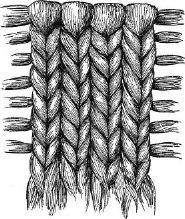
\includegraphics[scale=0.6]{./images/fig172}
\caption{Figurine from arizona. }
\end{figure}

\makeatother

\section{Epiloque}

We have managed to write a database, sort it, typeset its contents in a structured or freeform manner
and on the way we have documented the code using a form of \textit{literate programing.} On top which
other language expects you to code your own ifs and iteration routines? 
The amount of code we wrote is very minimal and competes with other modern languages. On top there is also a minimal commitment to using pre-defined commands.

Hope you had fun. Go and make beautiful
books.


\end{document}